\section{Part I -  Mathematical modeling}

In this section a mathematical model of the system, using the notations from Figure (\ref{fig:heli}) and Figure (\ref{fig:heli2}), will be derived to form the entry point for the rest of the assignment

\begin{figure}[H]
	\centering
	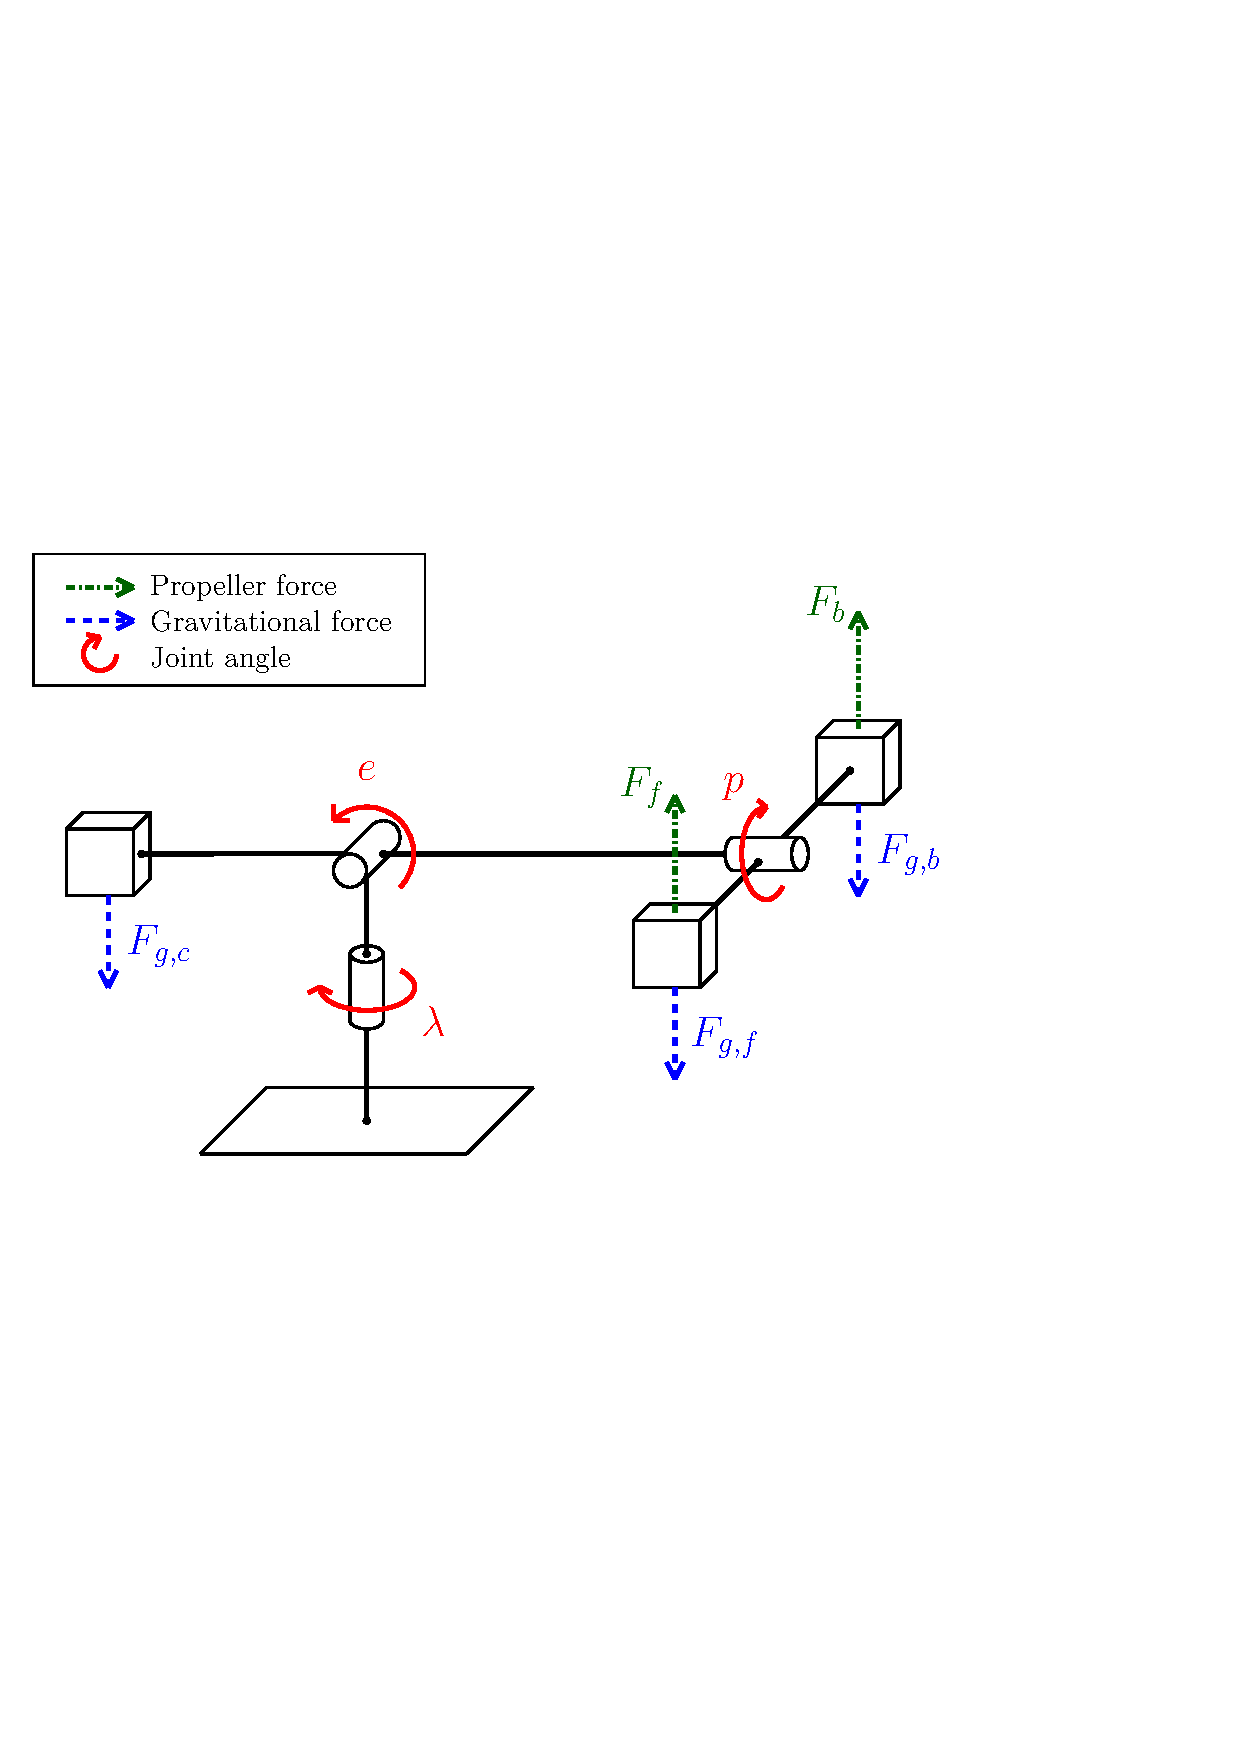
\includegraphics[width=0.9\textwidth]{figures/forces.pdf}
	\caption{Figure of the helicopter model from the assignment }
\label{fig:heli}
\end{figure}

\begin{figure}[H]
	\centering
	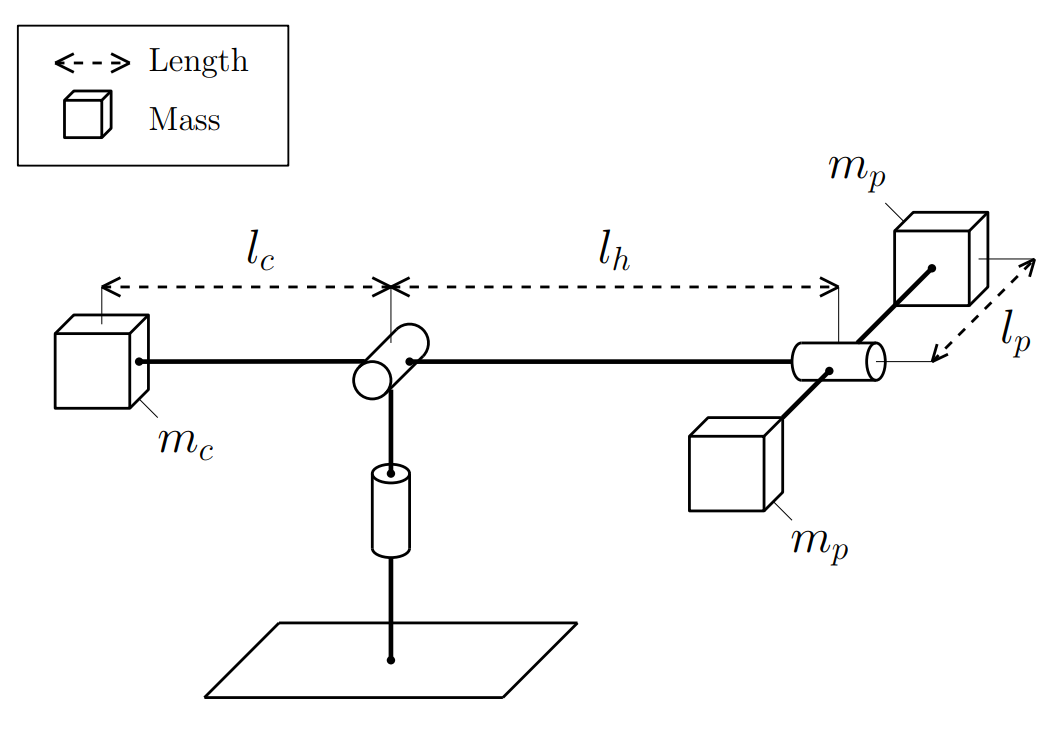
\includegraphics[width=0.9\textwidth]{figures/modelofmassesandlength}
	\caption{Figure of masses and lengths as shown in the assignment }
\label{fig:heli2}
\end{figure}


\subsection{Problem 1}
At first the equations of motion must be computed for the pitch angle $p$, the elevation angle $e$, and the travel angle $\lambda$. The moments of inertia about the pitch, elevation and the travel axes are denoted as $J_p$, $J_e$ and $J_{\lambda}$.
We are given the following relations:

\begin{equations}
    \begin{align}
        F_f &= K_f V_f \\ 
        F_b &= K_f V_b \\
        V_s &= V_f+V_b \\
        V_d &= V_f-V_b
    \end{align}
\end{equations}
\newline
where the propeller forces for the front and back propeller are given by $F_f$ and $F_b$, respectively. $K_f$ is the motor force constant which we will calculate a value for later in the assignment. 

Further on we can derive the following relations:

\begin{equations}
    \begin{gather}
        \sum M_p=J_p\alpha_p=J_p\ddot{p}=(F_f-F_b)l_p-(F_g_,_f-F_g_,_b)l_p \nonumber \\
        J_p\ddot{p}=K_fV_dl_p \nonumber \\
        L_1=K_fl_p \nonumber \\
        J_p\ddot{p}=L_1V_d \label{eq: 1}  \\
        f_p = \ddot{p} = \frac{L_1}{J_p} \cdot V_d \label{eq: fp}
    \end{gather}
\end{equations}


\begin{equations}
    \begin{gather}
       \sum M_e = J_e\alpha_e = J_e\ddot{e}= (F_f+F_b)l_h \cdot cos(p) - (F_g_,_f+F_g_,_b)l_h\cdot cos(e)+F_g_,_cl_c\cdot cos(e) \nonumber \\
       J_e\ddot{e}=K_fV_sl_hcos(p)-2m_pgl_hcos(e)+m_cgl_ccos(e) \nonumber \\
       L_2=m_cgl_c-2m_pgl_h \nonumber \\
       L_3=K_fl_h \nonumber \\
       J_e\ddot{e}=L_2cos(e)+L_3V_scos(p) \label{eq: 2} \\
       f_e = \ddot{e} = \frac{L_2}{J_e} \cdot cos(e) + \frac{L_3}{J_e} \cdot V_s cos(p) \label{eq: fe}
    \end{gather}
\end{equations}

\begin{equations}
    \begin{gather}
        \sum M_\lambda=J_\lambda\alpha_\lambda=J_\lambda\ddot{\lambda}=(F_f+F_b)l_h(-sin(p))cos(e) \nonumber \\
        J_\lambda\ddot{\lambda}=-K_fV_sl_hsin(p)cos(e) \nonumber \\
        L_4=-K_fl_h \nonumber \\
        J_\lambda\ddot{\lambda}=L_4V_ssin(p)cos(e) \label{eq: 3} \\
        f_\lambda = \ddot{\lambda} = \frac{L_4}{J_\lambda} \cdot V_s sin(p)cos(e) \label{eq: fl}
    \end{gather}
\end{equations}

\newline
\newline

At first we tried with a gain for $V_d$ only, but the helicopter wouldn't lift. Hence we added a gain of 8 for $V_s$ to finally make it lift. After this we tried to find the gain that gave us the best ''feel of control'' for $V_d$. After trying different values between 0.2 and 2 we ended up at 0.8. We also changed the sign of the gains to get a better correlation between the helicopter's motion and the joystick.  
After this we could compare the behavior of the helicopter with the model and the linearized model. Notice that $e$ is influenced by $p$ so that the helicopter drops slightly when the pitch turns, compared to $p$ being 0. This is because $\ddot{e}$ is given by $K_2 \cdot cos(p)$ and not only $K_2$ as described in the linearized model. However its not a very big difference, and as long as $p$ doesn't change too rapid the regulator for $e$ takes care of the error. The linearized model is quite good, but does not fit completely. 


%%%%%%%%%%%%%%%%%%%%%
\subsection{Problem 2}
We want to linearize the equations of motion around the point $(p,e,\lambda)^T = (p^*, e^*, \lambda^*)^T$ with $p^*=e^*=\lambda^*=0$. In an equilibrium point of the system when $\dot{p}=\dot{e}=\dot{\lambda}=0$, that yields $\ddot{p}=\ddot{e}=\ddot{\lambda}= 0$. In order to determine $V_s^*$ and $V_d^*$ we combine this information with (\ref{eq: fp}) and (\ref{eq: fe}) and get:

\begin{center}
\begin{equations}
    \begin{align}
        0 = L_1V_d^* \quad \Rightarrow \quad V_d^* &= 0 \\
        0 = L_2cos(0)+L_3V_s^*cos(0) \quad \Rightarrow \quad V_s^* &= \frac{-L_2}{L_3}
        \end{align}
\end{equations}

\begin{center}
    \begin{equations}
        x = \begin{bmatrix} p \\ e \\ \lambda \end{bmatrix}, \quad 
        u = \begin{bmatrix} V_s \\ V_d \end{bmatrix}, \quad
        x^* = \begin{bmatrix} 
        p^* \\ e^* \\ \lambda^* 
        \end{bmatrix} = 
        \begin{bmatrix} 
        0 \\ 0 \\ 0 
        \end{bmatrix} , \quad 
        u^* = \begin{bmatrix} 
        V_s^* \\ V_d^* 
        \end{bmatrix} = 
        \begin{bmatrix} 
        \frac{-L_2}{L_3} \\ 0 
        \end{bmatrix}
    \end{equations}
\end{center}

\end{center}

\newpage
To simplify further analysis, a coordinate transformation that has its equilibrium point in the origin is introduced:

\begin{center}
    \begin{bmatrix} \tilde{p} \\ \tilde{e} \\ \tilde{\lambda} \end{bmatrix} =
        \begin{bmatrix} p \\ e \\ \lambda \end{bmatrix} -
            \begin{bmatrix} p^* \\ e^* \\ \lambda^* \end{bmatrix}, \quad
            \begin{bmatrix} \tilde{V_s} \\ \tilde{V_d} \end{bmatrix} = 
        \begin{bmatrix} V_s \\ V_d \end{bmatrix} -
    \begin{bmatrix} V_s^* \\ V_d^* \end{bmatrix}
\end{center}

\begin{center}
    \begin{equations}
        p^* = e^* = \lambda^* = 0 \quad \Rightarrow \quad p = \tilde{p}, \quad e = \tilde{e} \quad \text{and} \quad \lambda = \tilde{\lambda}
    \end{equations}
\end{center}

\begin{center}
\begin{bmatrix} V_s \\ V_d \end{bmatrix} \quad = \quad
\begin{bmatrix} \tilde{V_s} - \frac{L_2}{L_3} \\ \tilde{V_d} \end{bmatrix}
\end{center}
\\
The system equations can now be written as:

\begin{equations}
	\begin{align}
    f_p = \ddot{\tilde{p}} &= \frac{L_1}{J_p} \cdot \tilde{V_d} \\
	f_e = \ddot{\tilde{e}} &= \frac{L_2}{J_e} cos(\tilde{e}) + \frac{L_3}{J_e} cos(\tilde{p}) (\tilde{V_s} - \frac{L_2}{L_3}) \\
	f_\lambda = \ddot{\tilde{\lambda}} &= \frac{L_4}{J_\lambda}(\tilde{V_s} - \frac{L_2}{L_3})sin(\tilde{p})cos(\tilde{e})
	\end{align}
\end{equations}
\\

Linearization of the system around $(\tilde{p}, \tilde{e}, \tilde{\lambda})^T = (0,0,0)^T$ and $(\tilde{V_s}, \tilde{V_d}) = (0,0)^T$ gives the following $\bm{A}$ and $\bm{B}$ matrices:
\\


\begin{equations}
    \begin{center}
        \bm{A} = \begin{bmatrix} \frac{\partial f_p}{\partial p} & \frac{\partial f_p}{\partial e} & \frac{\partial f_p}{\partial \lambda} \\ 
        \frac{\partial f_e}{\partial p} & \frac{\partial f_e}{\partial e} & \frac{\partial f_e}{\partial \lambda} \\ 
        \frac{\partial f_\lambda}{\partial p} & \frac{\partial f_\lambda}{\partial e} & \frac{\partial f_\lambda}{\partial \lambda}
        \end{bmatrix} _{(x=x^*, u=u^*)} = \begin{bmatrix} 0 & 0 & 0 \\
        \frac{L_3}{J_e}(-sin(p)) & \frac{L_2}{J_e}(-sin(e)) & 0 \\
        \frac{L_4}{J_\lambda} V_s cos(p)cos(e) & \frac{L_4}{J_\lambda} sin(p)(-sin(e)) & 0 
        \end{bmatrix} _{(x=x^*, u=u^*)}
    \end{center}
\end{equations}

\begin{equation}
        = \begin{bmatrix} 0 & 0 & 0 \\ 0 & 0 & 0 \\ \frac{L_4}{J_\lambda} V_s^* & 0 & 0 \\ \end{bmatrix} = 
        \begin{bmatrix} 0 & 0 & 0 \\ 0 & 0 & 0 \\ K_3 & 0 & 0 \end{bmatrix}
\end{equation}
\\
\begin{equations}
    \begin{center}
        \bm{B} = \begin{bmatrix} \frac{\partial f_p}{\partial V_s} & \frac{\partial f_p}{\partial V_d} \\ 
        \frac{f_e}{\partial V_s} & \frac{\partial f_e}{\partial V_d} \\ 
        \frac{\partial f_\lambda}{\partial V_s} & \frac{\partial f_\lambda}{\partial V_d} \\
        \end{bmatrix} _{(x=x^*, u=u^*)} = \begin{bmatrix} 0 & \frac{L_1}{J_p} \\
        \frac{L_3}{J_e} \cdot cos(p) & 0 \\
        \frac{L_4}{J_\lambda} \cdot sin(p)cos(e) & 0 
        \end{bmatrix} _{(x=x^*, u=u^*)} 
    \end{center}
\end{equations}
    
\begin{equation}
    = \begin{bmatrix} 0 & \frac{L_1}{J_p} \\ \frac{L_3}{J_e} & 0 \\ 0 & 0 \end{bmatrix} = \begin{bmatrix} 0 & K_1 \\ K_2 & 0 \\ 0 & 0 \end{bmatrix}
\end{equation}

\newpage
Which gives the konstants $K_2$, $K_2$ and $K_3$ the following values:

\begin{center}
    \begin{equation} \label{eq: k1k2k3}
        K_1 = \frac{L_1}{J_p}, \quad K_2 = \frac{L_3}{J_e}, \quad K_3 = \frac{L_4}{J_\lambda} V_s^*  
    \end{equation}
\end{center}
\\
%%%%%%%%%%%%%%%%%%%%%
\subsection{Problem 3}
The helicopter is difficult to control when using only feed-forward control. By changing the gain on the input from the joystick, the helicopter responded faster and behaved better, but was still hard to control. \\
\\*
The physical behaviour of the system compared to the simplified mathematical model will not be correct for all possible cases. External physical effects as friction, drag, ground effects etc. was not taken into account in our simplified model, equation (\ref{eq: 1}), (\ref{eq: 2}) and (\ref{eq: 3}). A model of the Simulink diagram can be seen in Figure (\ref{fig:P1p3}).

%%%%%%%%%%%%%%%%%%%%%
\subsection{Problem 4}

By measurement we found $V^{*}_s$ = 7$\frac{N}{V}$, and $K_f$ was now able to be calculated to be 0.9911. 
Because the arm of the helicopter was starting $-30^{\circ}$ below the equilibrium point, we subtracted -30 from the elevation to get the equilibrium point where we wanted it to be;
horizontal. 


